% Introduction

\pdfbookmark[1]{Introduction}{Introduction}

\chapter{Methodology}
\label{chap:methodology}

\begin{flushright}{\slshape    
If it disagrees with experiment, it's wrong.\\ 
In that simple statement is the key to Science.} \\ \medskip
--- Richard Feynman~\cite{Feynman:1965}
\end{flushright}


\bigskip

% Mention that models are all fundamentally wrong (required by other chapter)
The success of natural sciences lies in their great emphasis on the role of
quantifiable data and their interplay with models. Data and models are both
necessary for the progress of our understanding: data generate stylized facts
and put constraints on models. Models on the other hand are essential to
comprehend the processes at play and how the system works. If either is missing,
our understanding and explanation of a phenomenon are questionable. This issue
is very general, and affects all scientific domains, including the study of
cities.\\

Until recently, the field of urban economics essentially consisted in untested
laws and theories, unjustified concepts that supersede empirical
evidence~\cite{Bouchaud:2008}. Without empirical validation, it is not clear
what these models teach us about cities. The tide has turned in recent years,
however: the availability of data is increasing in size and specificity, which
has led to the discovery of new stylized facts and opened the door to a new
science of cities~\cite{Batty:2013}. Yet, the situation is not perfect: while
the recent deluge of data have triggered the apparition of many empirical
analyses, in the absence of convincing models to explain these regularities, it
is not always clear what we learn about cities.

In this chapter, we will try to specify what we mean by model, and explain with
a concrete example why data analysis is not enough understand the behaviour of
systems.


\section{Of models and theories}

\subsection{For what purpose?}
\label{sub:why_bother_}

As scientific sceptics often like to remind us, all models, all theories are
wrong. But surely, there must be some interest in models to make them deserve
the months, sometimes years of work that scientist devote to them. 

Models' two main functions are, broadly speaking, to understand, and to predict.
The benefits linked with the ability to predict the behaviour of a system need
not be recounted. Understanding is a more complicated notion, and a
philosophical discussion of the concept lies far beyond the scope of this
thesis. Roughly, to understand is to untangle the mechanisms involved so as to have a
simplified, barebone description of the processes that shape the system.\\

%%Dificulties with social sciences
%How can we explain, then, the difference between social sciences and natural
%ciences? Say, between economics and physics. Why, if the reductionist approach
%is also to function with social systems, don't we have anything nearly as trong
%a result as in the natural sciences? Clearly not because people are less
%intellectually capable of handling difficult problems. Quite the
%contrary, actually. One thing that jumps to your face when overlooking tebooks
%in physics and textbooks in Geography, or in economics, is the difficulty of the
%questions asked. The natural world is a complex realm as well, and there is no
%reason to believe that the social world should be any more complicated (even
%free minds obey to the law of large numbers when put together! And who tells you
%electrons do not have a free mind too?). But the questions physics asks are
%ridiculously simple, in comparison to what social scientists ask. In a way,
%physicists have this natural advantage that Nature is a somewhat less immediate
%reality to us, it is easier to distanciate oneself from physical phenomena than
%it is from social phenomena. The problem with social sciences (if we can call
%this a problem), is to try to solve complex questions because they are
%\emph{important to us}. 

%Clearly, in some fields, economics being one of them, sociolog closely following
%despite Bourdieu's criticism of the link between politics and sociology, this is
%exactly what happening. Because they are asked to `make more money', `save the
%conomy' or to justify such and such policy, these sciences have been preoccupied
%with very high level, very complex questions that could be subdivided into tens,
%hundreds, even more, simpler, more specific questions. They were asked to build
%a rocket too soon. Successful approaches (with a few exceptions, see
%thermodynamics) in physics were bottom-up approaches: by knowing the mecanisms
%behind different phenomena, we were able to influence them, and combine them to
%make objects that are more and more intricate. Top-down approaches rarely work,
%because our brains are somehow not wired not handle very complex questions. But
%we are cursed in the field of social sciences, because we are aware of the
%top-down kind of questions, while you cannot aim at inventing a rocket before
%knowing the basics of gravity. At least not seriously. There is something very
%paradoxical in today's society in the very simple fact that while very complex
%questions (regulate the economy, bringing full employment...) get massive
%attention from funding agencies, while science-fiction-like projects such as
%`inventing teletransportation' do not get a single euro from government
%agencies. For me, they are of the same order. A wish to go towards an ideal,
%allegedly better state of humanity, while not even knowing the mecanims on which
%we would need to play in order to get there. While not even knowing
%theoretically how to handle the problem. We only fund hard science projects that
%we know are feasible, that are just a matter of technicalities, at least in
%principle. Someone who would come up with the vague idea of writing a theory of
%everything without any serious basis to think this is what he is doing would
%have no chance to get any funding.\\

%This picture is obviously incomplete. Some models -- toy models for instance --
%do not aim at being correct from the beginning.



\subsection{Theory, not analogy}
\label{sub:theory_not_analogy}

Unfortunately, expressive words and metaphors are too often used as a substitute
for a real understanding of the system. But, however intellectually appealing
they are, metaphors are not a theory. For instance, what do we understand from
the comparison of cities with biological systems? What new knowledge do we gain?
Metaphors do not provide interesting ideas that are ready to be applied to a
specific field. Rather, they trigger very different ideas into different people,
which explains their recurrent success. Yet, what we need to highlight are
regularities, not similarities.\\

We also need to avoid models that are only loosely connected to reality, analogy
or metaphor. There is a lot of confusion, and little understanding to be gained
that way. In the words of Einstein, Podolsky and Rosen

\begin{quote}
    In a complete theory, there is an element corresponding to each element of
    reality.~\cite{Einstein:1935}
\end{quote}

In this thesis, we tried to make sure that most -- if not all -- elements
(variables) of our models are related to a quantity that is measurable. We also
paid a special attention to the rigour in the language used. We qualify
suggestions, by presenting them as such.  This kind of work may be less
suggestive, the vocabulary used less expressive, but it is a necessary step
towards a science of cities. We need to clear the language of unfruitful
metaphors and fill the gap with mechanisms.


%The approach taken in this thesis is reductionist, and we implicitely assume in
%our approach that every phenomenon can be reduced to a set of irreducible,
%fundamental laws. This should not be mistaken, however, for the opposite
%\emph{constructionist} view defended by Pierre-Simon de Laplace: the view that
%we can reconstruct the entire universe from a finite set of fundamental
%laws~\cite{Anderson:1972}. 
%History of Physics tends to prove to us that, in fact, all theories \emph{are}
%effective theories -- in the sense that they are only true at a given scale. Too
%aproximate when our measuring apparatus are able to probe nature more into
%details. The analogy here is clear: we need more data, more specific data first
%if we want to dig deeper into the reality of our societies, economies. We need
%more than our own eyes, more than our ears. We need social, economical
%telescopes.
%In a sense, this reduced reductionism is reassuring:  it means we do not need to
%have a full theoretical description of the human mind to say something about the
%actions of hundreds of thousands, a million of them.  In the same way we do not
%need string theory in order to explain the functioning of living organisms.
%Randomness is not to be understood as the opposite of rationality. Individuals
%may as well make perfectly rational, predictable decisions, we would still have
%to use a probabilistic approach. Particles are an extreme example of individuals
%with a rational behaviour, yet we describe their collective behaviour with
%statistical physics. Probabilities are not called for by the unpredictability of
%one's behaviour, but rather by the particular type of information that is
%important to us -- and that we can process.
%What tells us that the world is not more complex than the picture drawn by
%physical theories? That our best theories are only approximations that work a t
%a certain scale, but are plain wrong at others? Everything around us, and the
%history of physics itself. Reductionism does not imply renouncing to the world
%in its entirity and its complexity. Reductionism is merely a recognition of our
%limited capabilities, our possibility to grasp only the world tiny bit by tiny
%bit, approximation after approximation. It is not absurb to reduce the amount of
%information that is dealt with in theories, because this seems to be exactly how
%we are cognitively programmed to function. If our brains were able to embrace
%the world in all its details at once, one wouldn't need models, one would not
%need theories, one wouldn't need science. Observation would be synonymous 
%understanding.\\

\section{Quantitative stands for 'data'}
\label{sec:quantitative_stands_for_data_}

Richard Feynman's statement used as an epigraph in this chapter might be an
oversimplified, narrow view of what Science is and how it proceeds. It
nevertheless hits the nail right in the head, by isolating the core component of
what Science is: a tight relation with empirical analysis. Data are needed, at
first, to give us ideas about how the system works: stylized facts. We then
usually try to build a simplified version of the system, a model, that is able
to reproduce the stylized facts. Because of the simplification entailed, the
model highlights the most important features of the phenomenon and allows us to
understand the behaviour of the system. Finally, we use data again to test the
predictions of the model and assess its validity and/or limitations.

In this thesis, we adopt a quantitative approach to the the study of cities. In
other words, we extract information about urban systems using measured quantities: data. As we will argue in the next section,
however, data are not enough.


\subsection{Against data}
\label{sec:against_data}

In `Againt Method', the philosopher of science Paul Feyerabend argued against
the idea that Science proceeds through the application of a single, monolithic
method; what people usually call `The Scientific Method'~\cite{Feyerabend:1975}.
The reference is not innocent, and I will argue here that, although empirical
analysis constitutes the alpha and the omega of our enquiry for knowledge, data
are not enough.
There is common confusion, often innocent, that because data are at the core of
scientific enquiry, one only needs data analysis to understand how a system
works and predict its behaviour -- especially so when we have a lot of data. A
very extreme view of this statement has recently been put forth by Big Data
supporters. An article in the magazine `Wired'~\cite{Anderson:2008} recently
argued that the current deluge of data marked the end of Science as we know it.
That models were not necessary anymore, that they were to be replaced with the
extensive correlation analysis that a vast amount of data allow. This view is
completely misguided.\\

For one, pure data analysis is, at best, a myth: as Pierre Duhem argued in
$1906$~\cite{Duhem:1997}, all empirical observations are theory-laden. That is,
they are necessarily affected by the theoretical presuppositions held by whoever
is making the observation. Measuring the population of a city, for instance,
presupposes that there are such objects as cities, and that we can delineate
them. A deluge of data does not relieve the investigator from defining the
objects she is studying, from implicitely thinking about the relation between
the different elements in the system.

Then, correlations are science, indeed. But they are rudimentary science, and
there is nothing new about them. Arguably, the reason why we are able to
function at all as individuals is because our brain is capable of computing
correlations all the time. Take chairs. Chairs are fairly simple objects. Yet,
they come in all kind of colors, material and shapes. And despite this
potentially infinite diversity, we are able to recognise a chair when we see
one. We also have a notion of what a chair is to be used for. Although we do not
ackowledge it often, we are capable of surprisingly high levels of abstraction
and generalisation. Because our brains correlate, all the time. 

Science starts with the observation of these regularities. For instance, that
the sun always appears at the same place and disappears in the opposite
directions. That seasons come and go regularly. That after the night always
comes the day. Are pure correlations useful? Yes, for limited applications. Do
they constitute science? No. Science is when one goes beyond the simple
observation of correlations, and tries to understand the mechanisms responsible
for the correlations we observe.\\

In short, data is not enough: we must build models, theories.


\subsection{An example: The law of metropolises}
\label{sec:an_example_the_law_of_metropolises}

\subsubsection{Statement}
\label{sub:statement}

The above discourse may seem a bit abstract, so let us observe the shortcomings
of pure data analysis on a simple example, related to cities.

Using the GEOPOLIS database, Moriconi-Ebrard and Pumain derived a general transversal rule about system
of cities, that they called \emph{law of metropolises}~\cite{Pumain:1997}. If we
note $P_U$ the urban population of systems of cities (here countries), and $P_1$ the size of
their largest city~\graffito{The original regularity was observed for what the
author calls 'metropolises', which are roughly equivalent to the largest city in
terms of population.}, we can
plot $P_1$ versus $P_U$ for all systems of cities and obtain the plot on
Figure~\ref{fig:metropolises}.

\begin{figure}
    \centering
    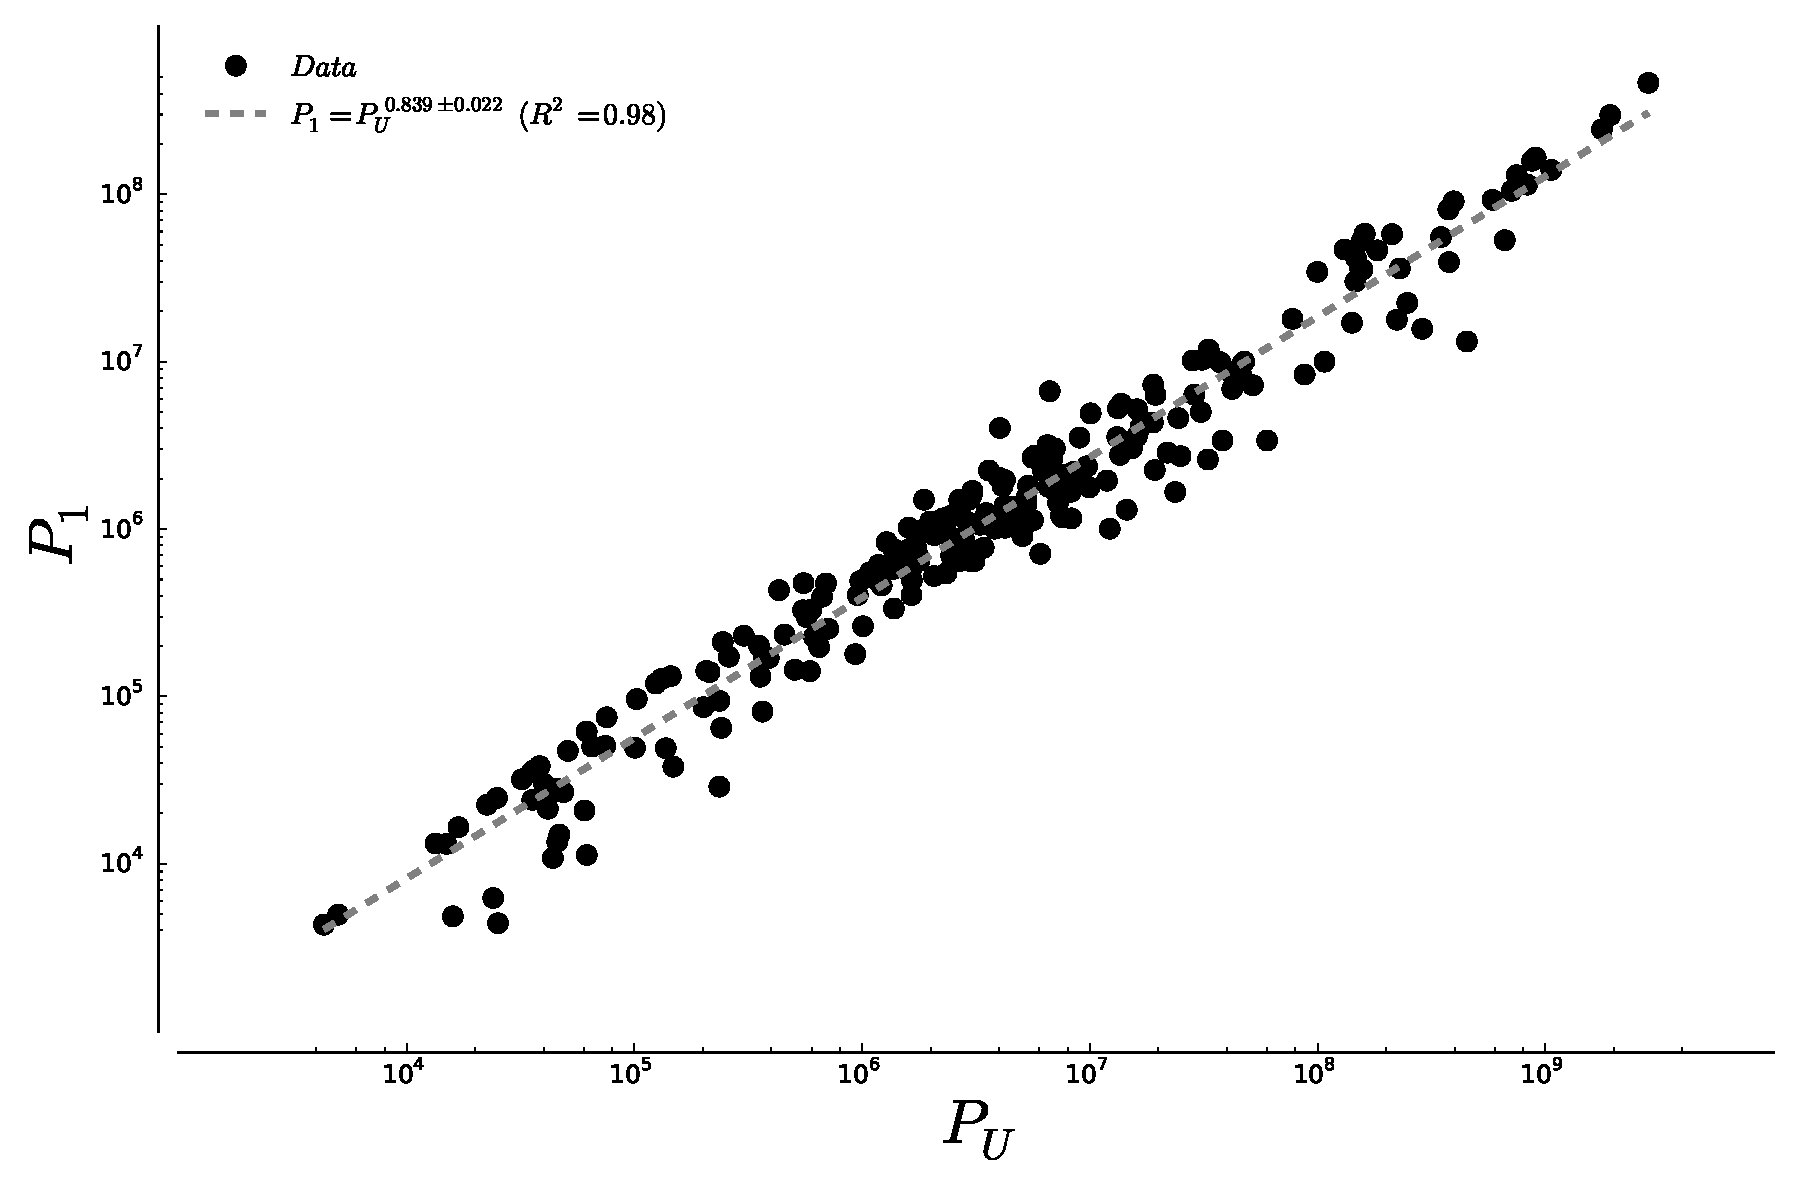
\includegraphics[width=\textwidth]{gfx/chapter-intro/law_metropolises.pdf}
    \caption{{\bf The law of metropolises.} Population of the largest city of
    systems of cities $P_1$ versus the total urban population $P_u$ in that
system. The dashed line shows the result of a powerlaw fit, whose exponent
agrees well with the one found in~\cite{Pumain:1997}. Data for the total urban
population and the population of the largest city of countries in the year
$2000$ were obtained from
the World Bank.\label{fig:metropolises}}
\end{figure}

Assuming a powerlaw relationship between the two quantities, one finds

\begin{equation}
    P_1 \sim P_U^{\,0.84}\:(r^2=0.98)
    \label{eq:metropolis}
\end{equation}

which agrees very well with the empirical data (for all years where data are
available). It is tempting, at first, to consider this as yet-another emprical
regularity exhibited by urban systems, and try to find a coherent interpretation
in geographical terms. However, as we will show, if we assume that the Auerbach-Zipf
law~\cite{Auerbach:1913,Zipf:1949} holds for each system of cities
individually

\begin{enumerate}
    \item We can derive a relation that fits the data as well as
        Eq.~\ref{eq:metropolis};
    \item The relation is not a powerlaw.
\end{enumerate}



\subsubsection{Deriving the `law of metropolises'}
\label{sub:deriving_the_law_of_metropolises_}

Let us consider a system of cities comprised of $N$ cities, with total
population $P_U$. The size of the largest city is noted $P_1$. We assume that
the distribution of city sizes follows the Auerbach-Zipf law, so that the city
of rank $r$ (the $r$th largest city) has a population

\begin{equation*}
    P_r = P_1\,r^{-\mu}
\end{equation*}

So the total population in the system of cities can be written

\begin{equation}
    P_U = \sum_{r=1}^N P_r = P_1\,\sum_{r=1}^{N} \frac{1}{r^\mu}
\end{equation}

If we assume that $\mu=1$, $P_U$ is given by the harmonic series, and thus

\begin{equation}
    P_U = P_1 \left[ \ln(N) + \gamma + O\left(\frac{1}{N}\right)\right]
\end{equation}

where $\gamma \approx 2.58$ is Euler's constant. This gives us a first relation
between $P_1$, $P_U$ and $N$.\\

Still using the assumption that the distribution of city size follows the
Auerbach-Zipf law with $\mu=1$, we can show (using extremal value
theory)~\cite{Clauset:2009} that on average\graffito{'Average' as in {\bf
ensemble average}} the size of the largest city is proportional to the total
number of cities

\begin{equation*}
    P_1 \propto N
\end{equation*}

Thus, when the number of cities in the system is large, $N \gg 1$ the following
relation holds 

\begin{equation}
    \boxed{P_1\,\ln(P_1) = P_U}
    \label{eq:metropolises_debunked}
\end{equation}

As one can see on Figure\ref{fig:metropolises_debunked}, the formula given by
Eq.~\ref{eq:metropolises_debunked} fit the data as well as the previous one.

\begin{figure}
    \centering
    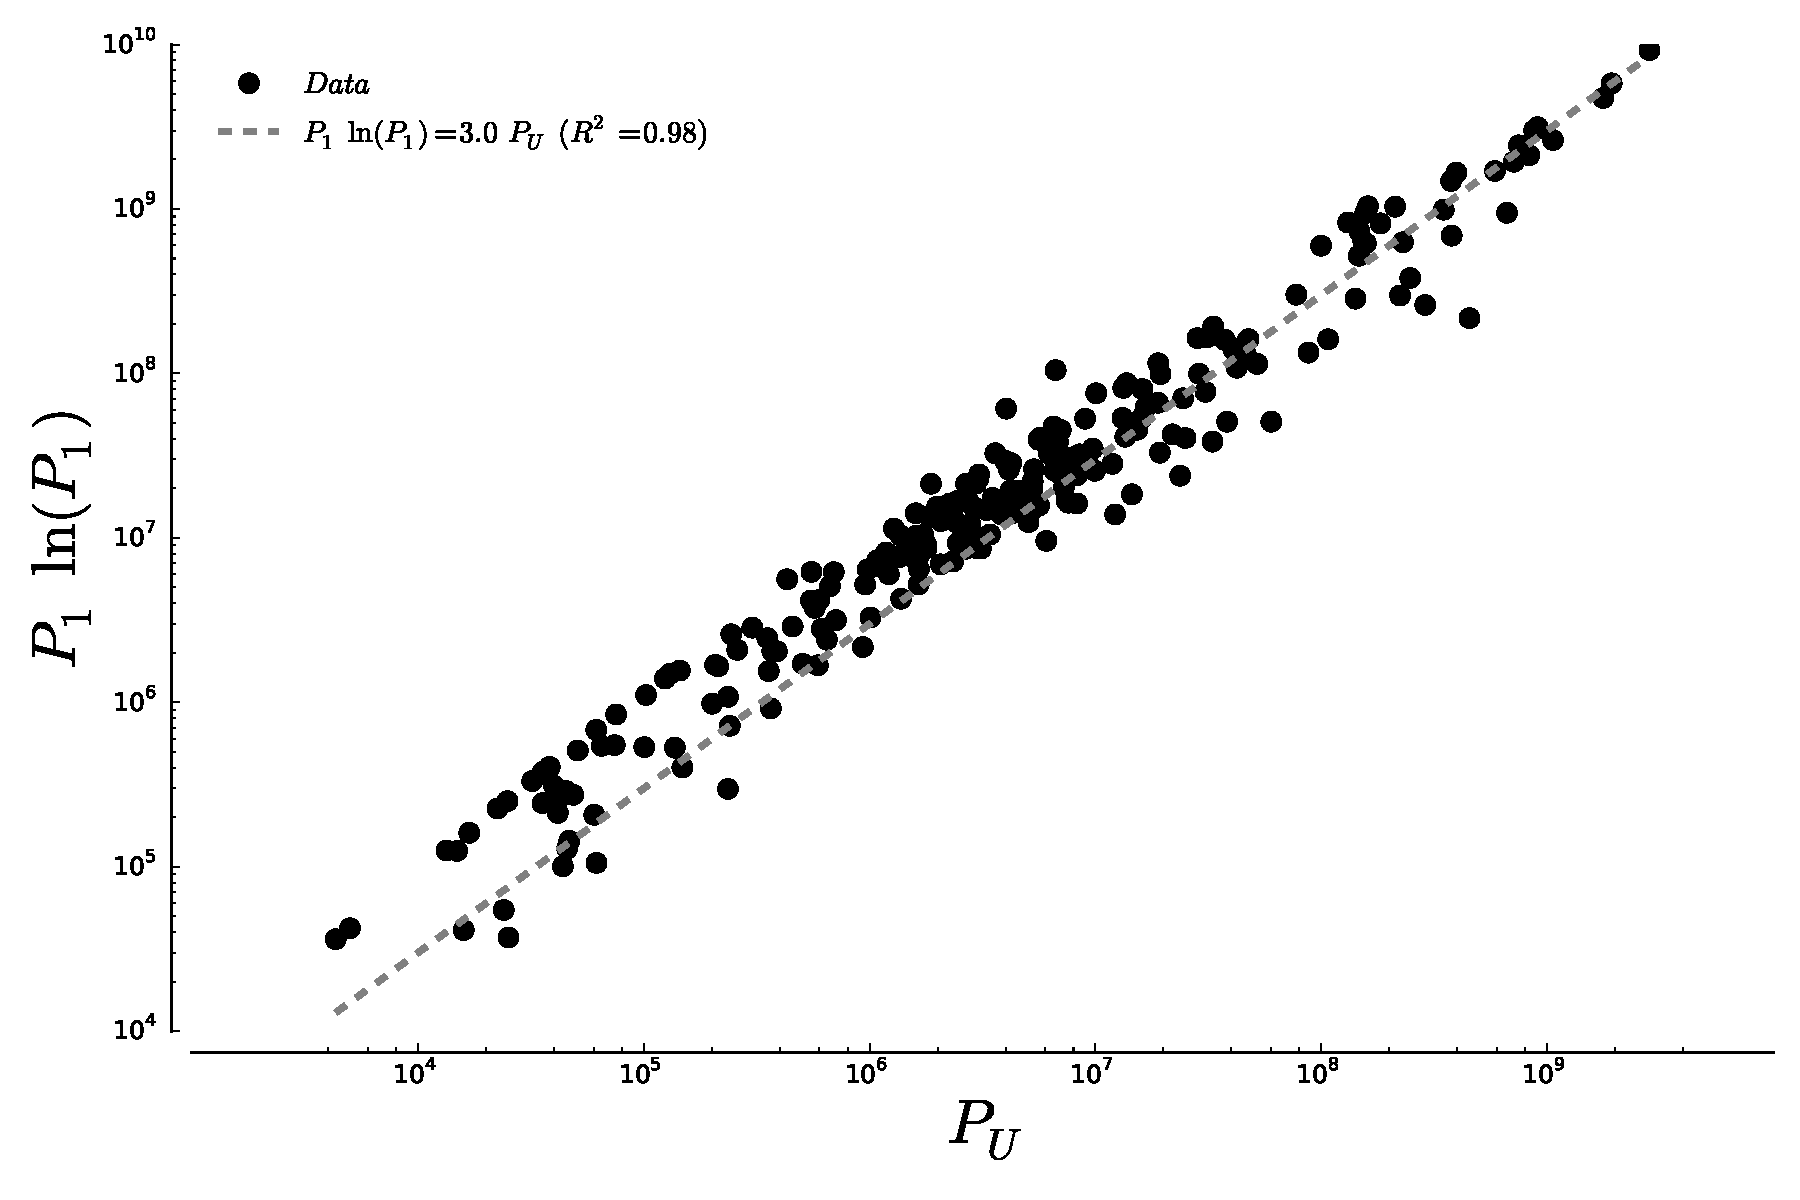
\includegraphics[width=\textwidth]{gfx/chapter-intro/law_metropolises_debunked.pdf}
    \caption{{\bf The law of metropolises revisited.} $P_1 \ln(P_1)$ versus the total urban population $P_u$ in that
system. The dashed line shows the result of a linear fit, which agrees as well
with the data as does the powerlaw relation assumed in~\cite{Pumain:1997}. Data for the total urban
population and the population of the largest city of countries in the year
$2000$ were obtained from
the World Bank.\label{fig:metropolises_debunked}}
\end{figure}


It is therefore impossible to determine which of
Eq.~\ref{eq:metropolis} or Eq.~\ref{eq:metropolises_debunked} describes the
`true' relation between $P_1$ and $P_U$ based on data analysis alone.
Nevertheless, the later finds a very simple explanation in the fact that cities
in systems of cities follow the Zipf-Auerbach law up to a good
approximation. In the absence of any theoretical explanation for the powerlaw
relationship and given the empirical equivalence of both forms, it
least-assuming to consider $P_1 \ln P_1 \sim P_u$.


\subsubsection{Lessons learned}
\label{sub:lessons_learned}

So, the \emph{law of metropolises} is not a fundamental relation.
This teaches us that, given the range of variation of the measured
quantities, it is very difficult to distinguish empirically a powerlaw
relationship from something qualitatively different such as $Y \ln Y \sim P$, as
recently argued by Shalizi in~\cite{Shalizi:2011}.
One should therefore be wary of interpreting empirical relationships,
like the one originally found in~\cite{Pumain:1997}, unless a mechanistic
explanation of the fitted relationship is provided. As shown above, what
was thought as a fundamental law might end up being trivial and without great
interest.

We will further discuss the limitations of data analysis in
Chapter~\ref{chap:scaling_implications}, after having studied scaling relationships.



